\documentclass[11pt, a4paper]{article}

\usepackage{graphicx}
\usepackage[margin=2cm,top=2cm,bottom=2cm]{geometry} % Adjust margins

\usepackage{url} % Required for \url{}
\usepackage{xcolor} % Required for specifying colors by name
\usepackage{subcaption}
\usepackage{hyperref}
\usepackage{float}
\usepackage[utf8]{inputenc} % Enable UTF-8 encoding
\usepackage{titlesec}
\usepackage{mfirstuc}
\usepackage{lipsum}
\usepackage{helvet}
\usepackage{changepage} % for the adjustwidth environment
\usepackage{fancyhdr}
\renewcommand{\familydefault}{\sfdefault}
\usepackage{caption}
\usepackage{multicol}


\begin{document}
\title{Bartlett RC11 2023-2024}
\author{Joris Putteneers}
\date{}
\maketitle
% first assignment

\section {Houdini Fundamentals}

This session covers the Houdini fundamentals. For the exercise, the following is expected:

\begin{itemize}
	\item Alter 2 of the example setups we covered during class. This means, add/remove a minimum of 2 nodes to a setup. Changing the parameters is not enough. Adding a Null SOP or adding unconnected nodes does not count.
	\item Describe in detail what exactly your setup is doing. Some important keywords and terminology are \textit{node, parameter, procedural, datatype, attribute, class, geometry, point, primitive, vertex, etc.}. Obviously, the example below cannot be used.
\end{itemize}

An example of such a description could be:

% Overview image
\begin{figure}[h]
	\centering
	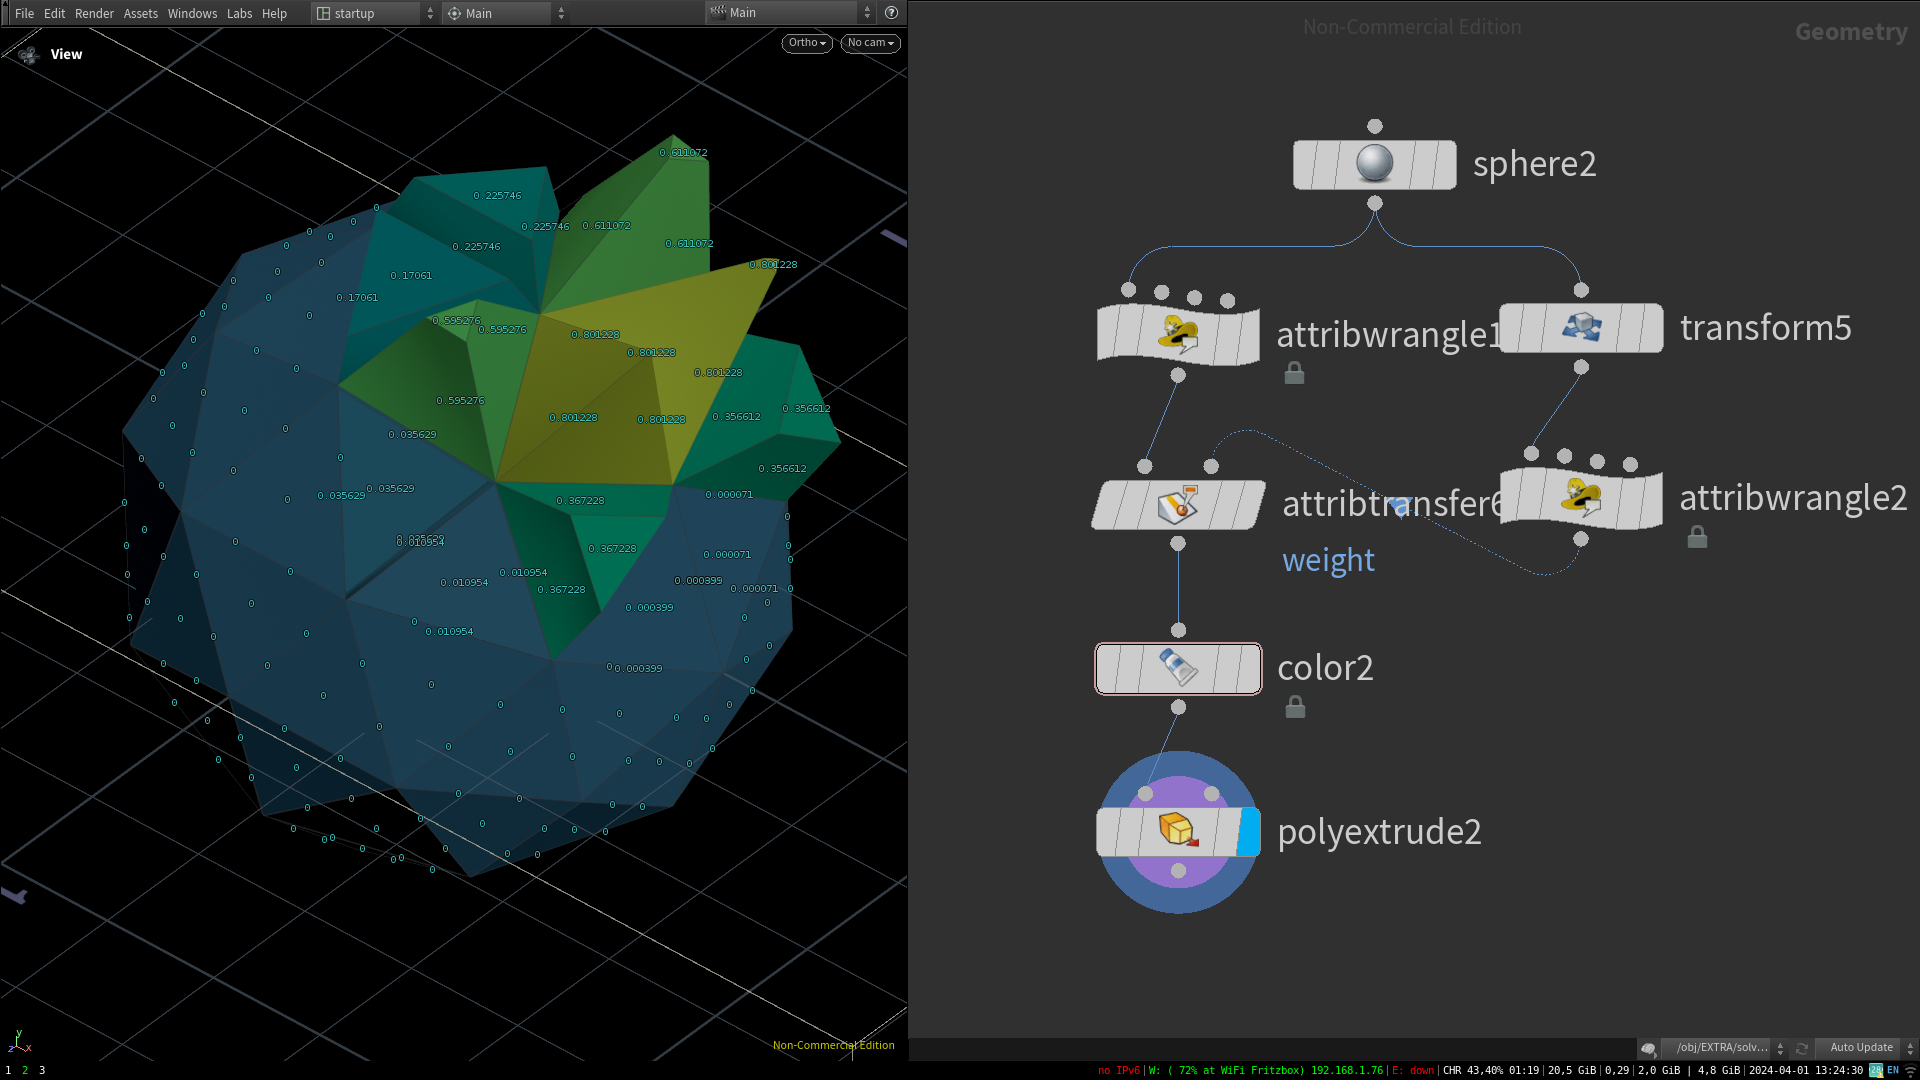
\includegraphics[width=\textwidth]{media/houdini_fundamentals_overview.png}
	\caption{Houdini Fundamentals: Setup 1 Overview}
	\label{fig:assignment1}
\end{figure}

\begin{minipage}[H!]{0.4\textwidth}
	\textbf{1: Sphere SOP} \newline 

 The "sphere" is of primitive type: polygon. One of the basic geometric data
types that contains points, primitives of type polygon, and vertices.  

\end{minipage}
\vspace{1pt}
\begin{minipage}[H]{0.6\textwidth}
	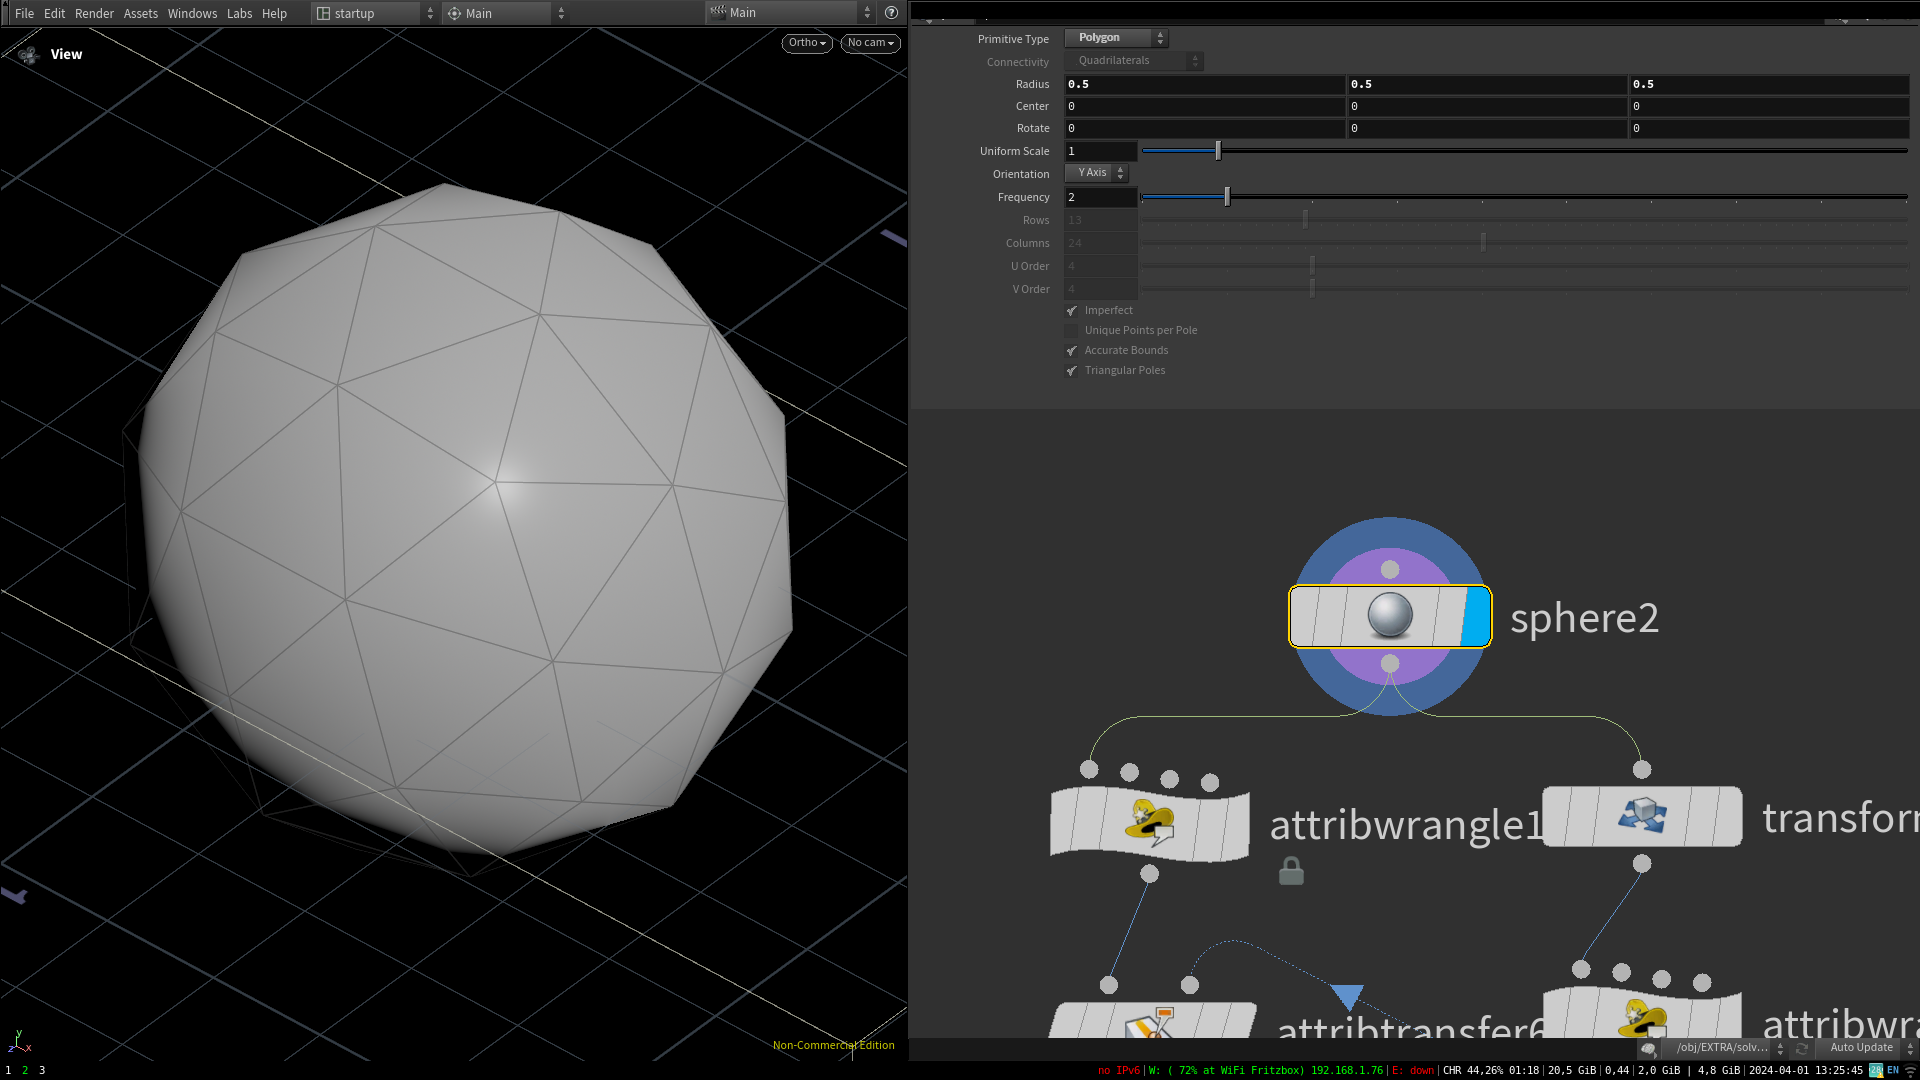
\includegraphics[width=1\textwidth]{media/houdini_fundamentals_1.png}
\end{minipage}



\begin{minipage}[H]{0.4\textwidth}
	\textbf{2: Attribute Wrangle SOP}\newline 

We create an "Attribute Wrangle" SOP, where we make a "weight" attribute. The
attribute is of type float as described by the "f@" declaration. The attribute
is set to run over primitives. This is because later in the node setup, we will
use a PolyExtrude node where we will need a primitive attribute to drive the
extrusion value. The value is set to 0 (which will be interpreted as 0.0
because of the float declaration) because later, we can interpolate between 0
and 1. 
	
 \end{minipage}
\vspace{1pt}
\begin{minipage}[H]{0.6\textwidth}
	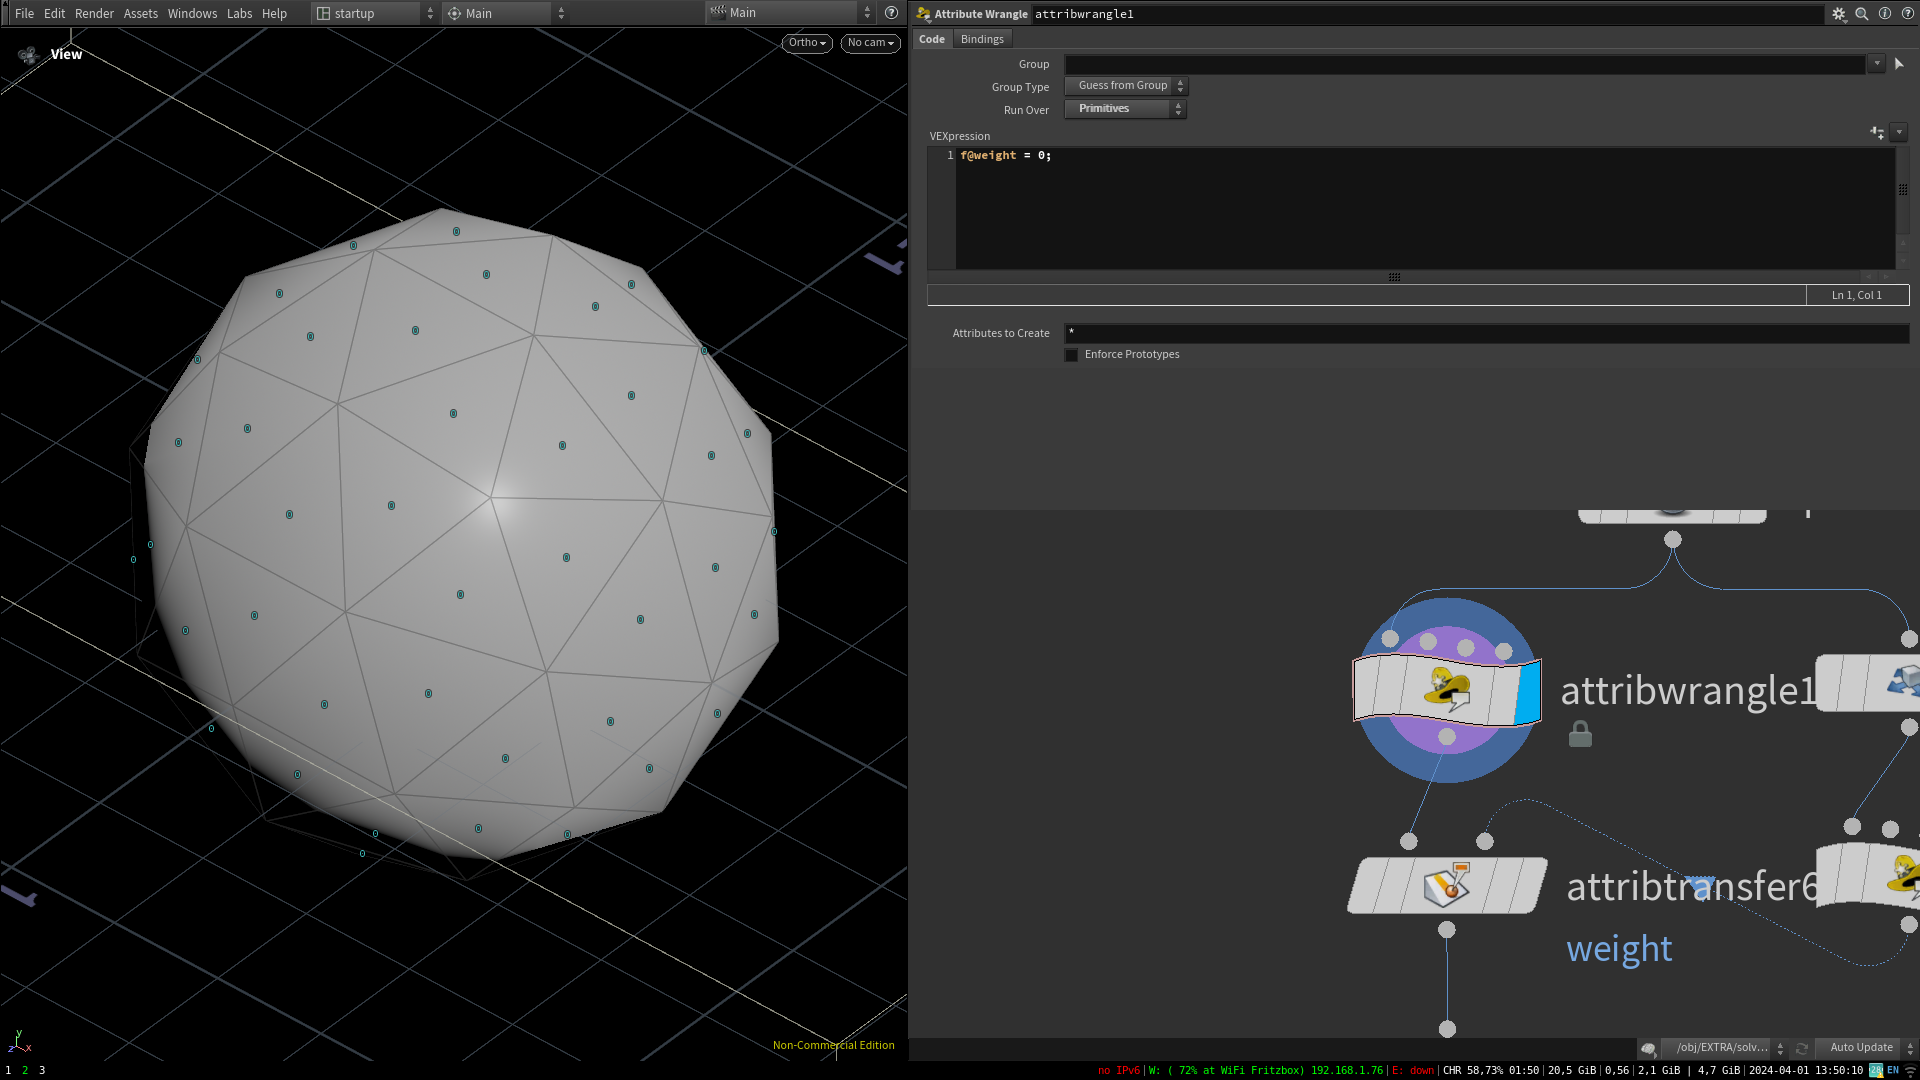
\includegraphics[width=1\textwidth]{media/houdini_fundamentals_2.png}
\end{minipage}


\vspace{10pt}

\begin{minipage}[H]{0.4\textwidth}
	\textbf{3: Transform SOP}\newline 

Then, we lay down a "Transform" SOP. This will be the attractor; it is just a
duplicate of the original sphere. The distance between this duplicate
(attractor) and the original sphere will dictate the final extrusion value. 
	
\end{minipage}
\vspace{1pt}
\begin{minipage}[H]{0.6\textwidth}
	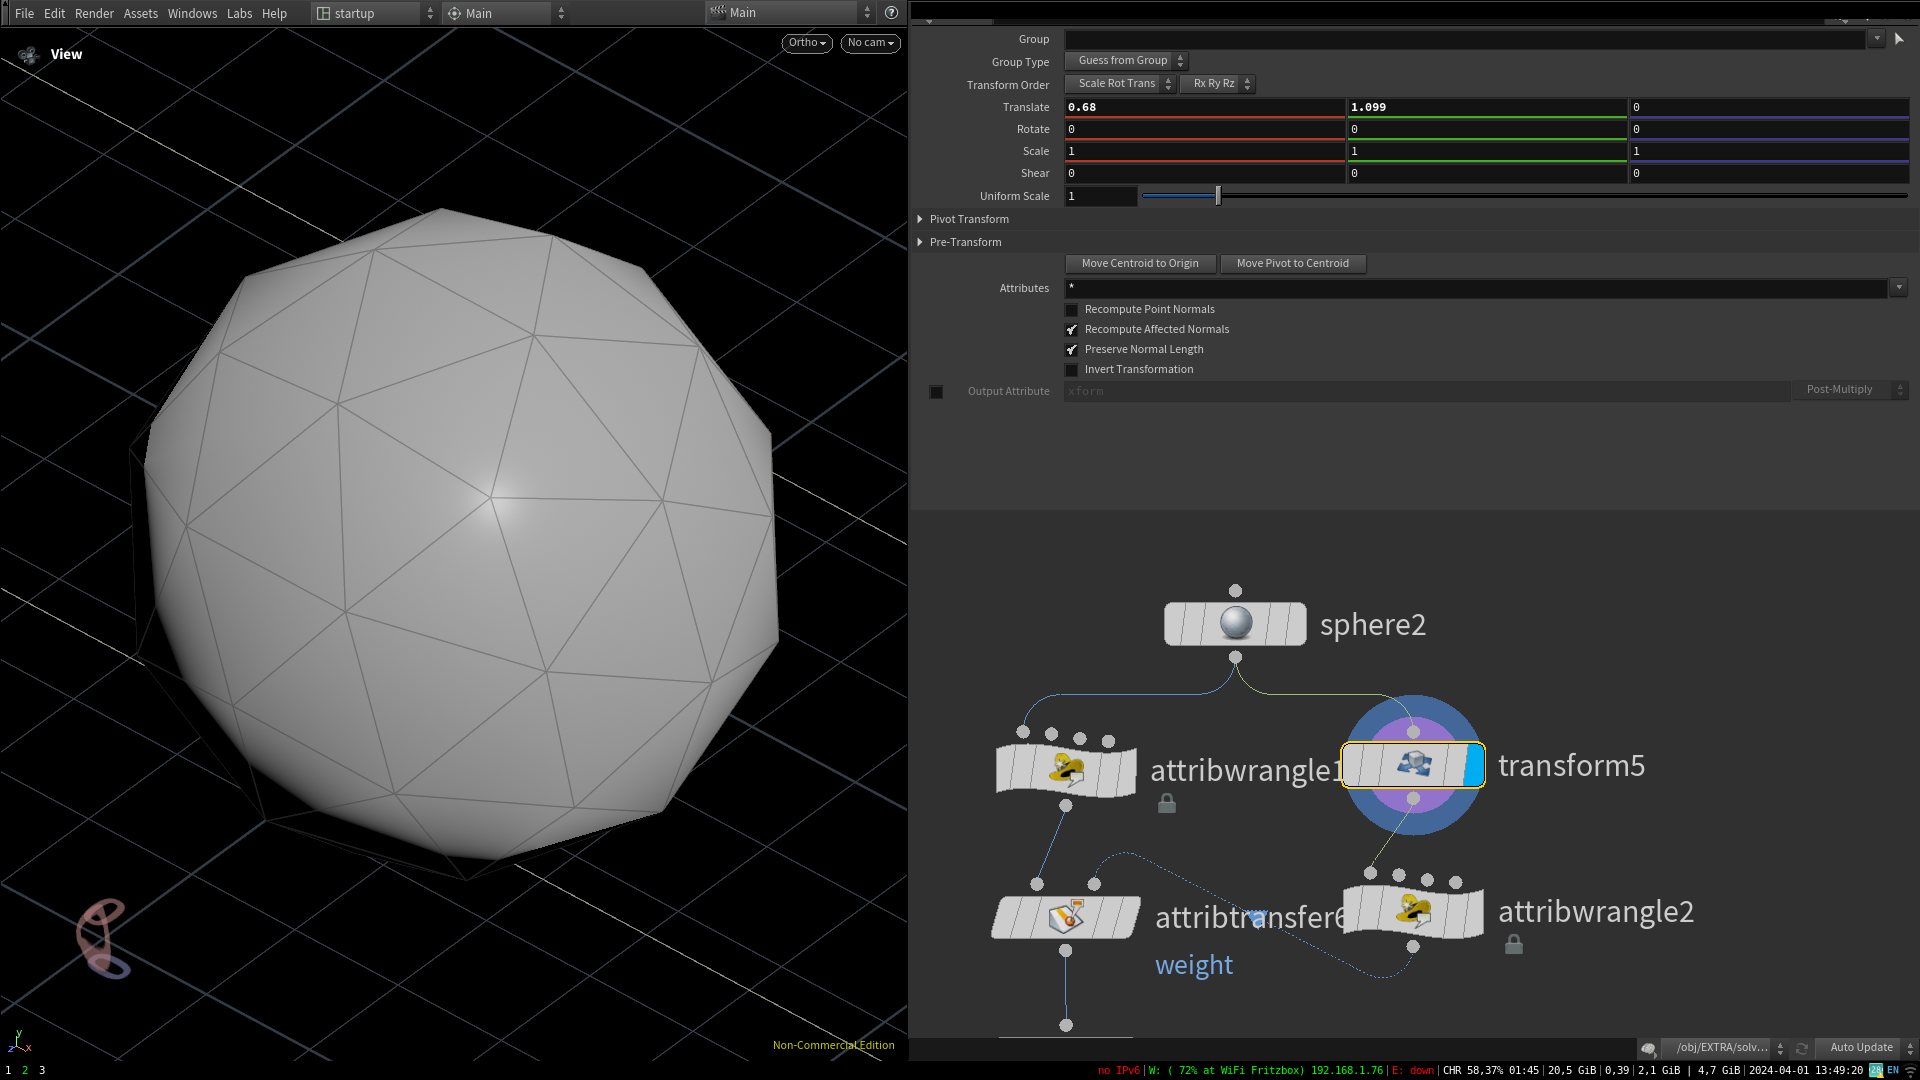
\includegraphics[width=1\textwidth]{media/houdini_fundamentals_3.png}
\end{minipage}


\begin{minipage}[H]{0.4\textwidth}
	\textbf{4: Attribute Transfer SOP}\newline 

The "Attribute Transfer" SOP uses the "weight" primitive attribute to write out
the distance value between the original sphere and the attractor. By setting
the original 'weight' attribute as float, we can have value interpolations
between 0 and 1. If we had set the weight attributes to integers, we could not
interpolate; the output values would be binary (0 or 1). 
 
\end{minipage}
\vspace{1pt}
\begin{minipage}[H]{0.6\textwidth}
	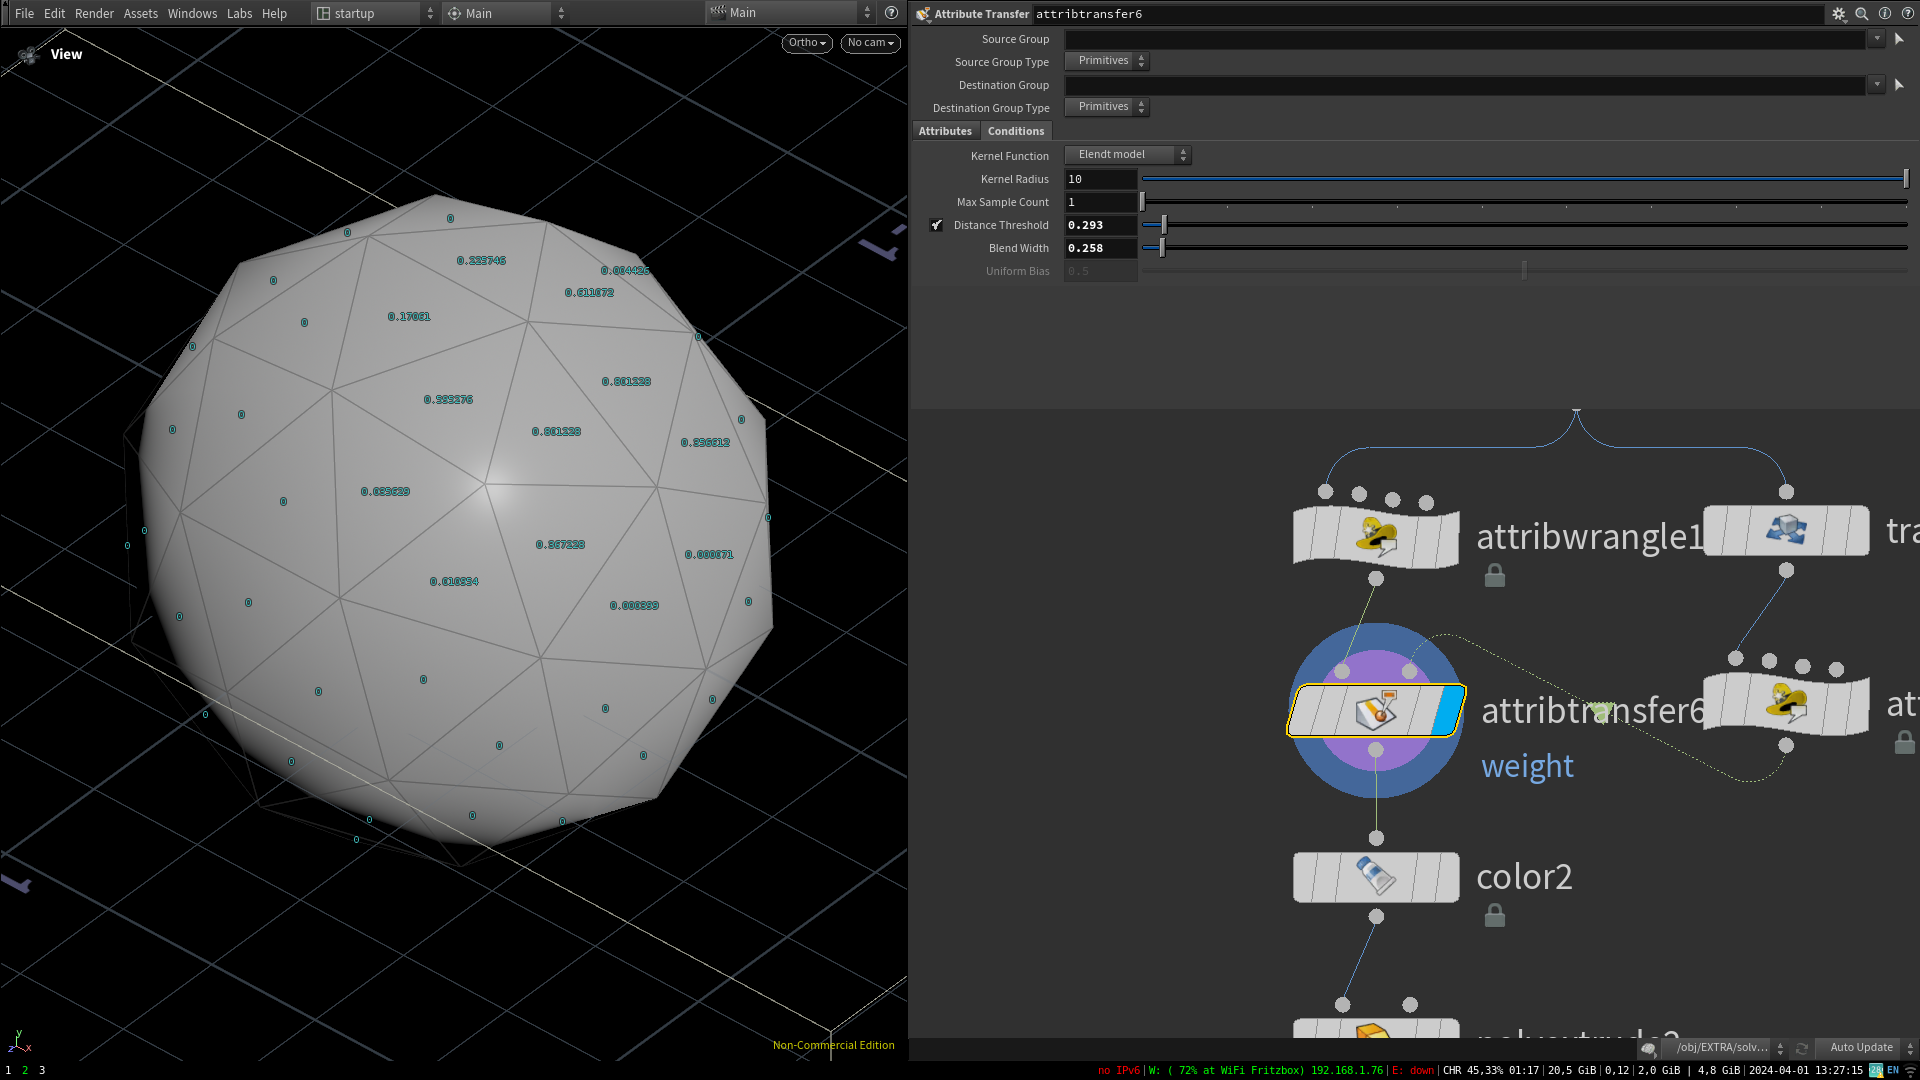
\includegraphics[width=1\textwidth]{media/houdini_fundamentals_4.png}
\end{minipage}


\begin{minipage}[H]{0.4\textwidth}
	\textbf{5: Attribute Wrangle SOP}\newline 
The same as the previous Wrangle SOP, only with the opposite value. The reason
we interpolate between 0 and 1 is because it is easier to work with normalized
values than arbitrary values. 
	
\end{minipage}
\vspace{1pt}
\begin{minipage}[H]{0.6\textwidth}
	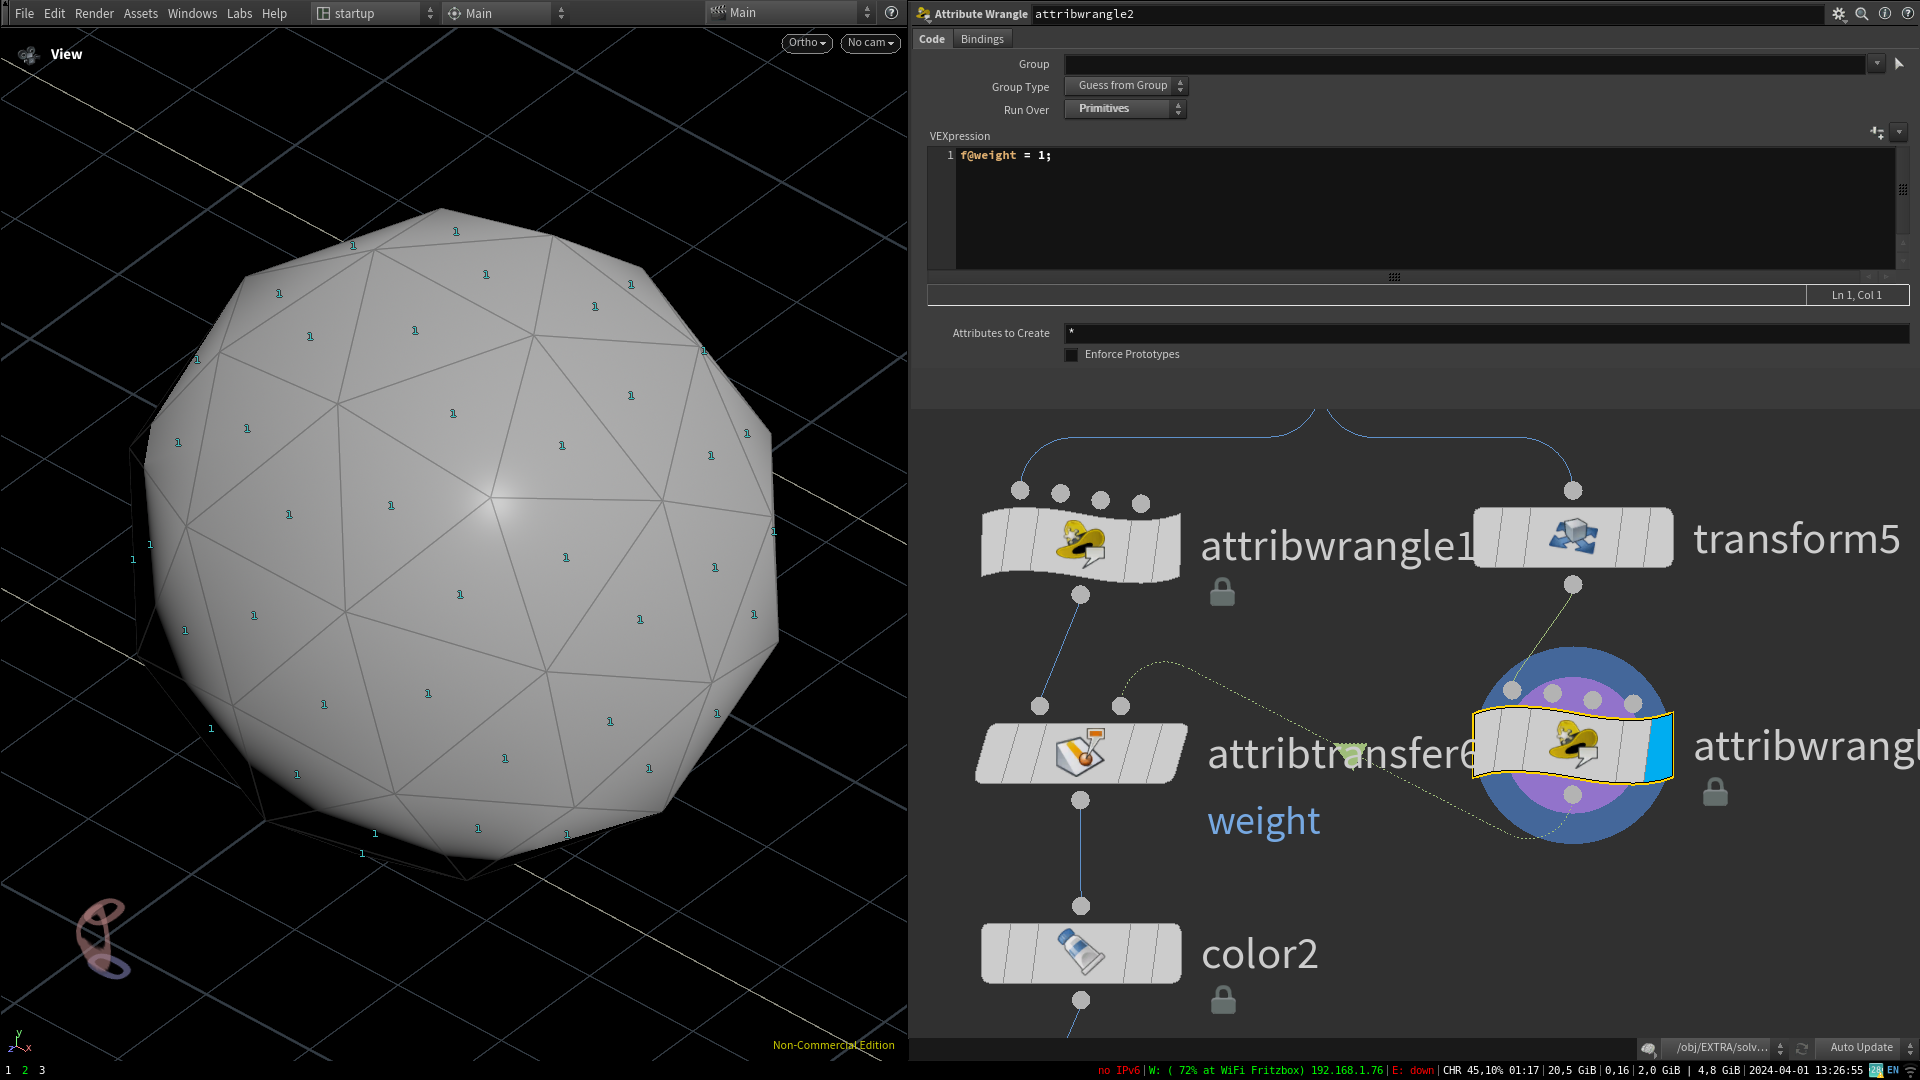
\includegraphics[width=1\textwidth]{media/houdini_fundamentals_5.png}
\end{minipage}


\begin{minipage}[H]{0.4\textwidth}
	\textbf{6: color SOP}\newline 
A visualisation of the "weight" primitive attribute according to the "viridis"
colorscheme. Because we normalized our values between 0 and 1, it is more stable
if we would ever change distances, or geometry inputs.
\end{minipage}
\vspace{1pt}
\begin{minipage}[H]{0.6\textwidth}
	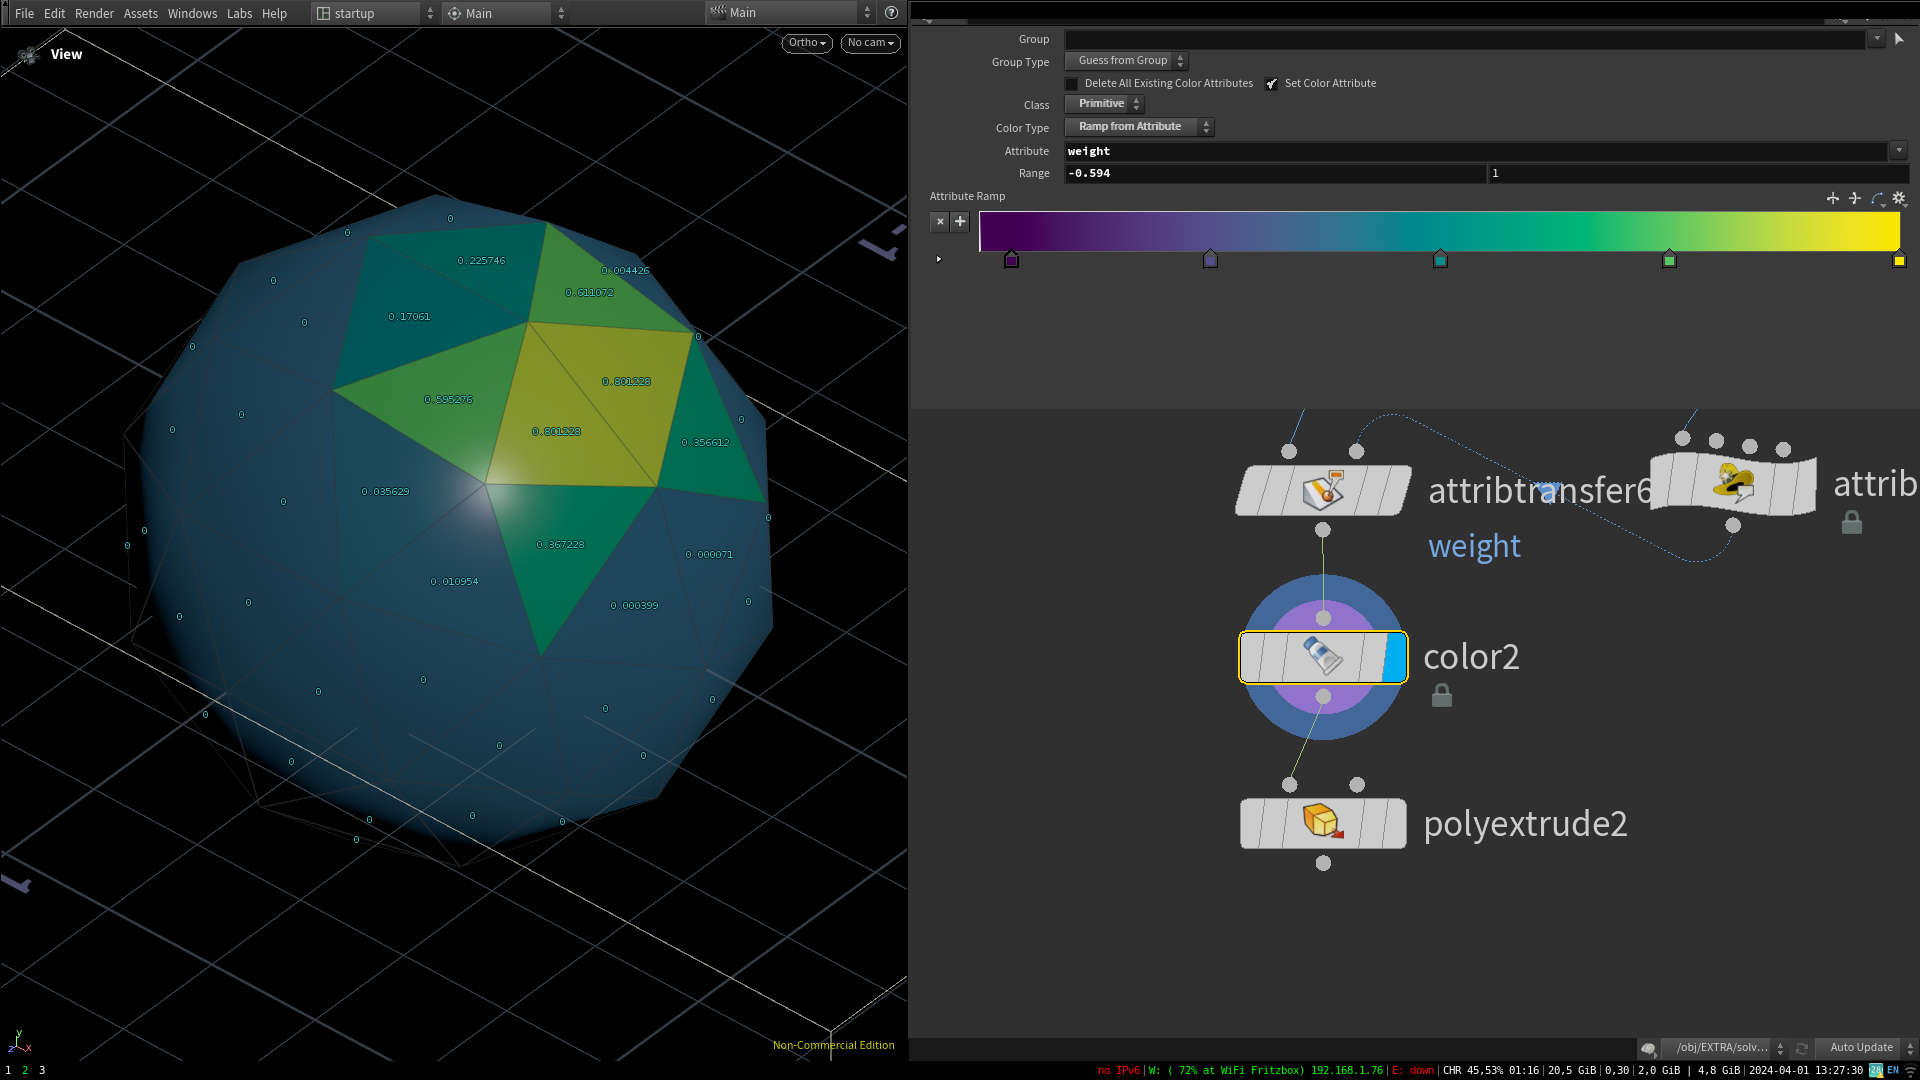
\includegraphics[width=1\textwidth]{media/houdini_fundamentals_6.png}
\end{minipage}



\begin{minipage}[H]{0.4\textwidth}
	\textbf{6: PolyExtrude SOP}\newline 
Using the "weight" value in d"distance scale", we use the weight value as a
multiplier of the extrusion value. If we set the distance value to 0, the
extrusion is 0 (0 x weight). If we set the distance value to 1, we get the full
weight value as extrusion (1 x weight) \end{minipage}
\vspace{1pt}
\begin{minipage}[H]{0.6\textwidth}
	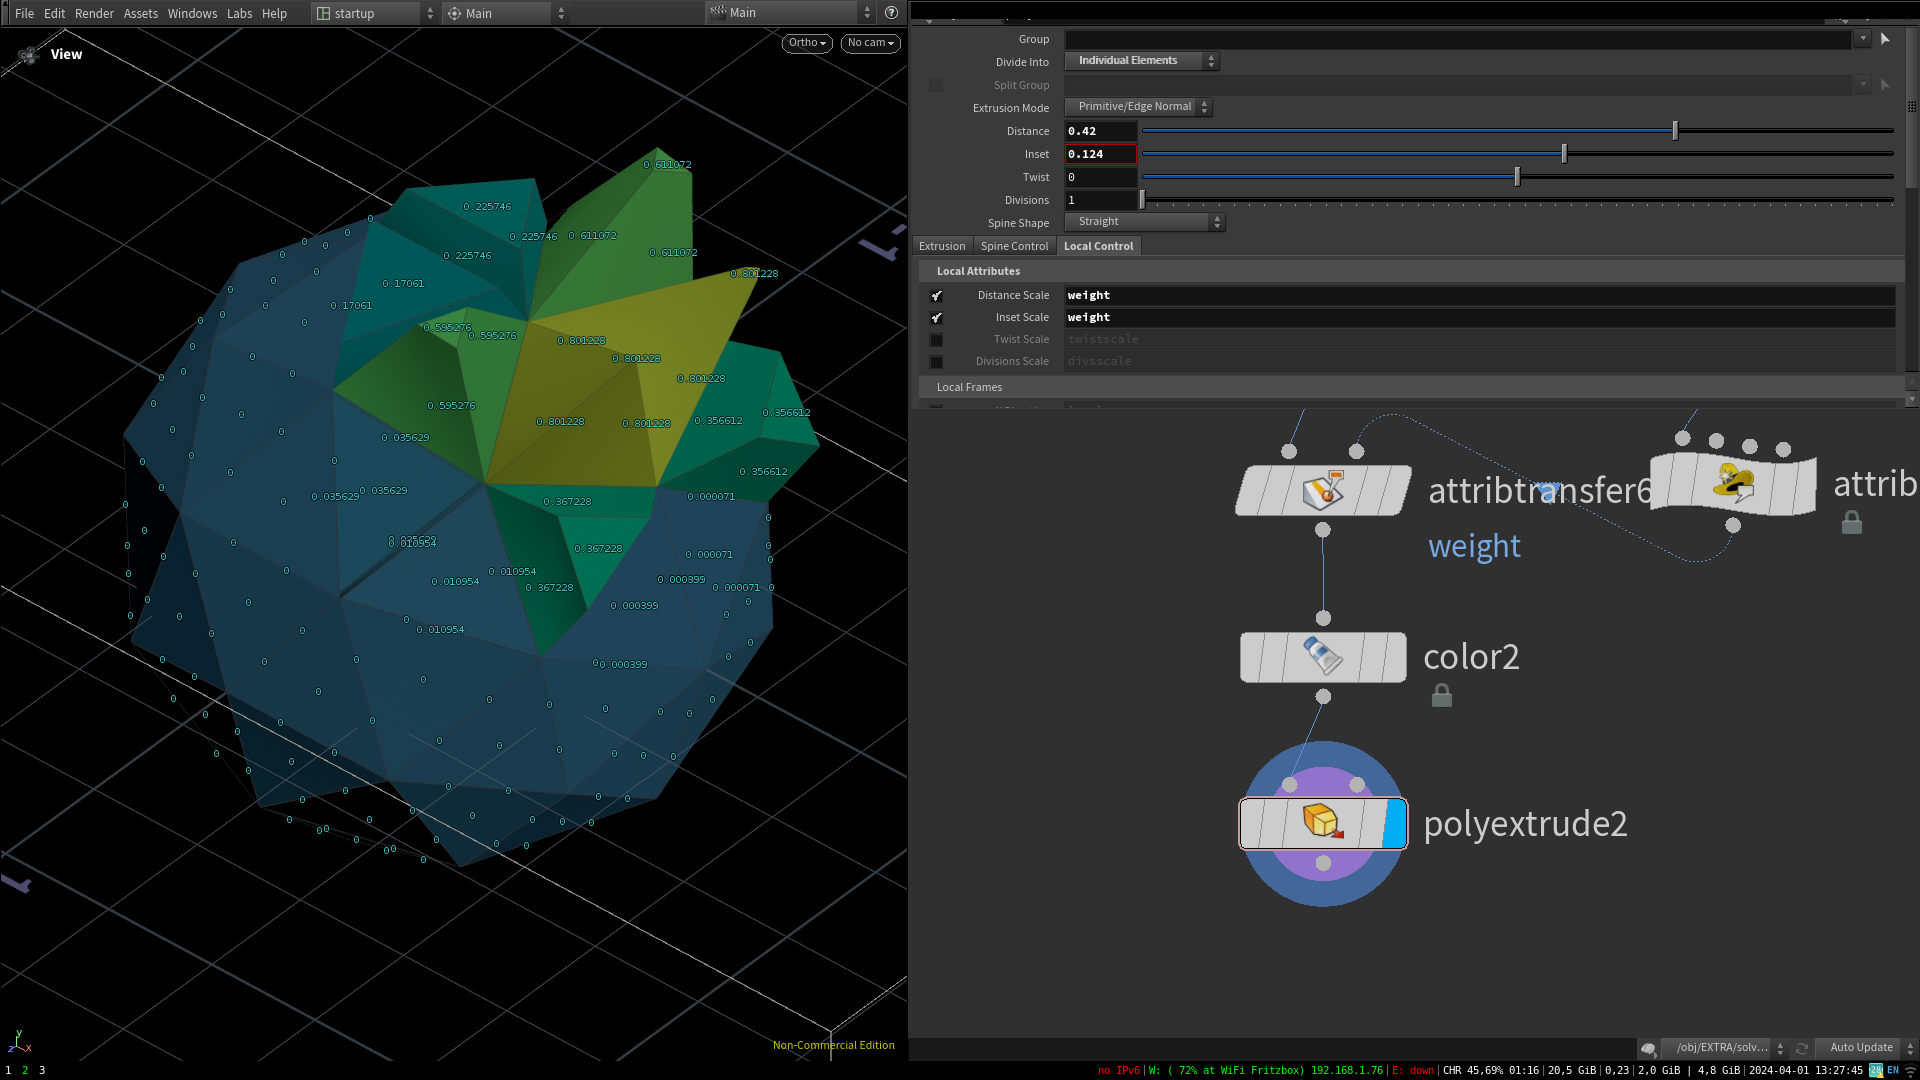
\includegraphics[width=1\textwidth]{media/houdini_fundamentals_7.png}
\end{minipage}



\newpage
\section {Visualizing GPS and Image Metadata}

This session covers how to overlay your Google Maps trajectories with images in
Houdini. For the assignment, the following is expected:

\begin{itemize}
	\item Load in your own images and GPS data. 
	\item Generate a series of images depicting your travels.
	\item A short description of the procedure. 
\end{itemize}

An example of such a description would be :

\begin{figure}[H]
	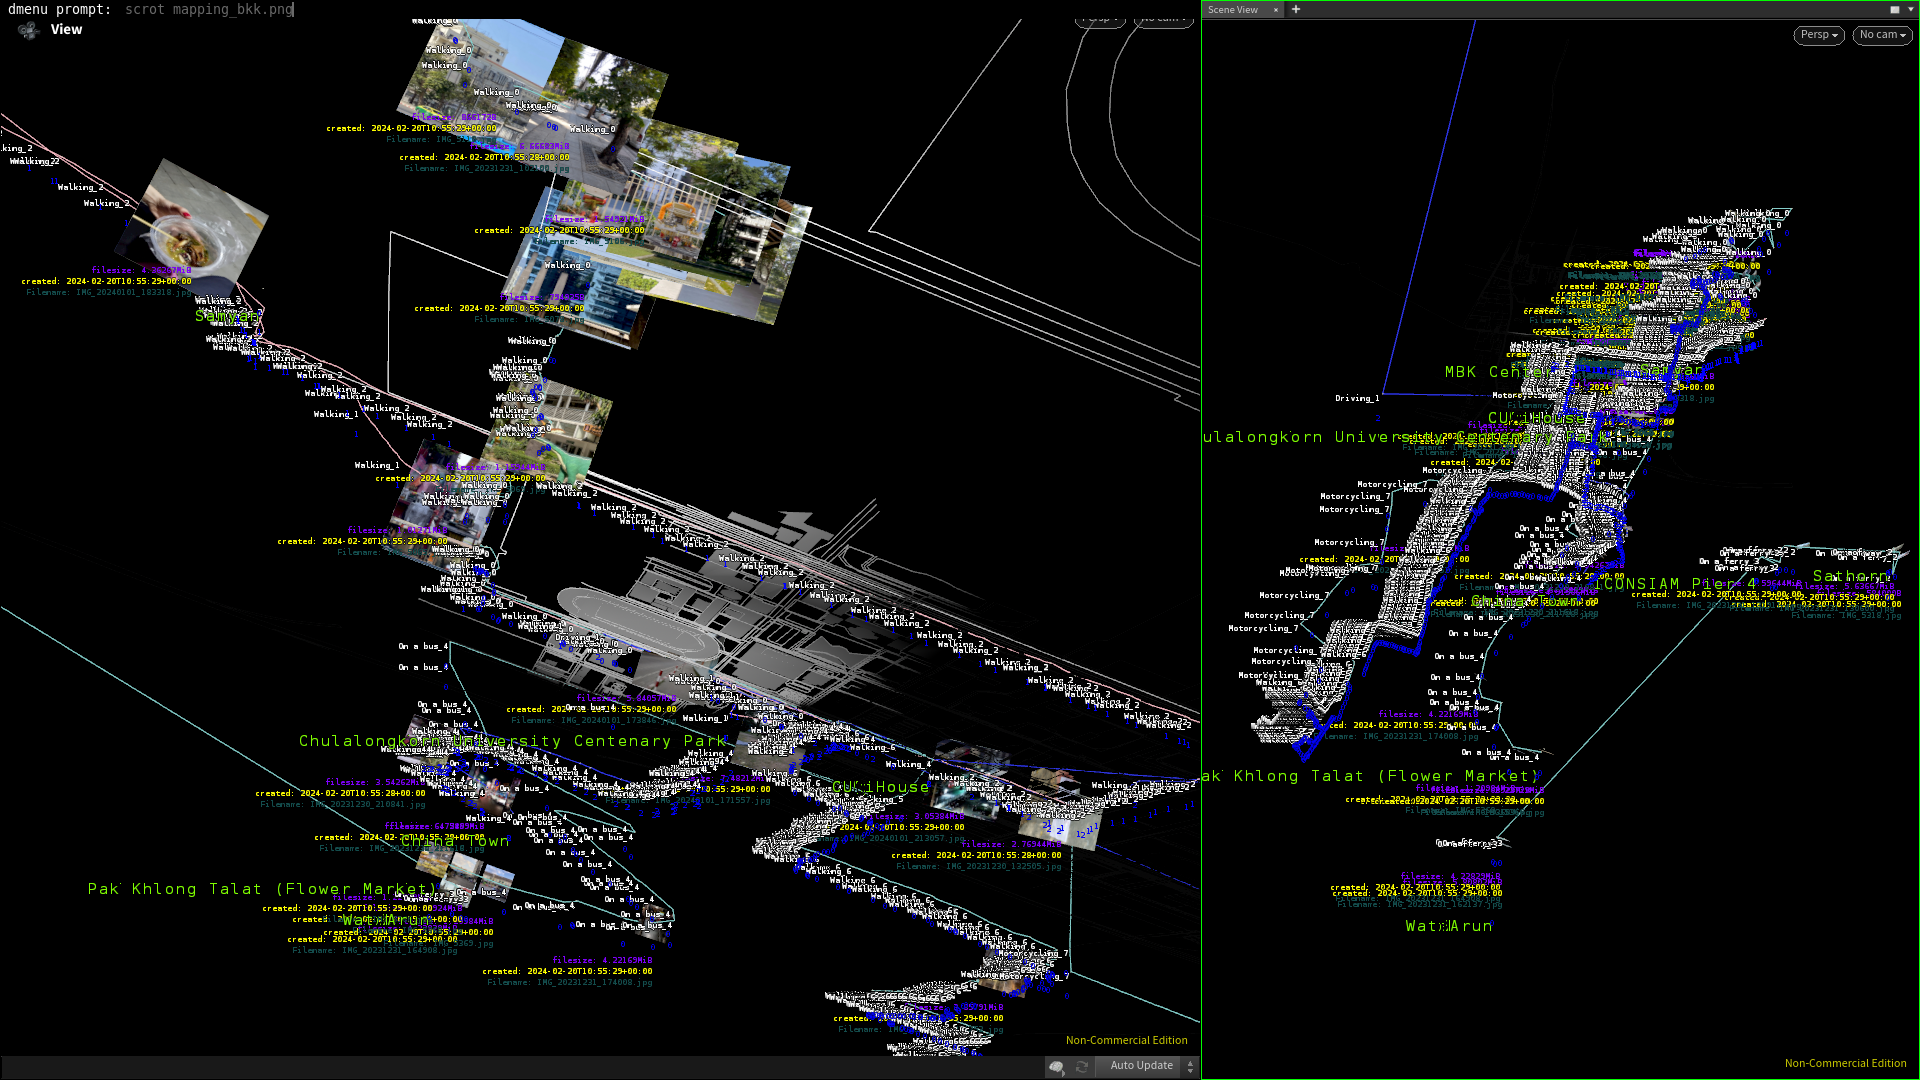
\includegraphics[width=\textwidth]{media/mapping_bkk.png}
\end{figure}

\begin{figure}[H]
	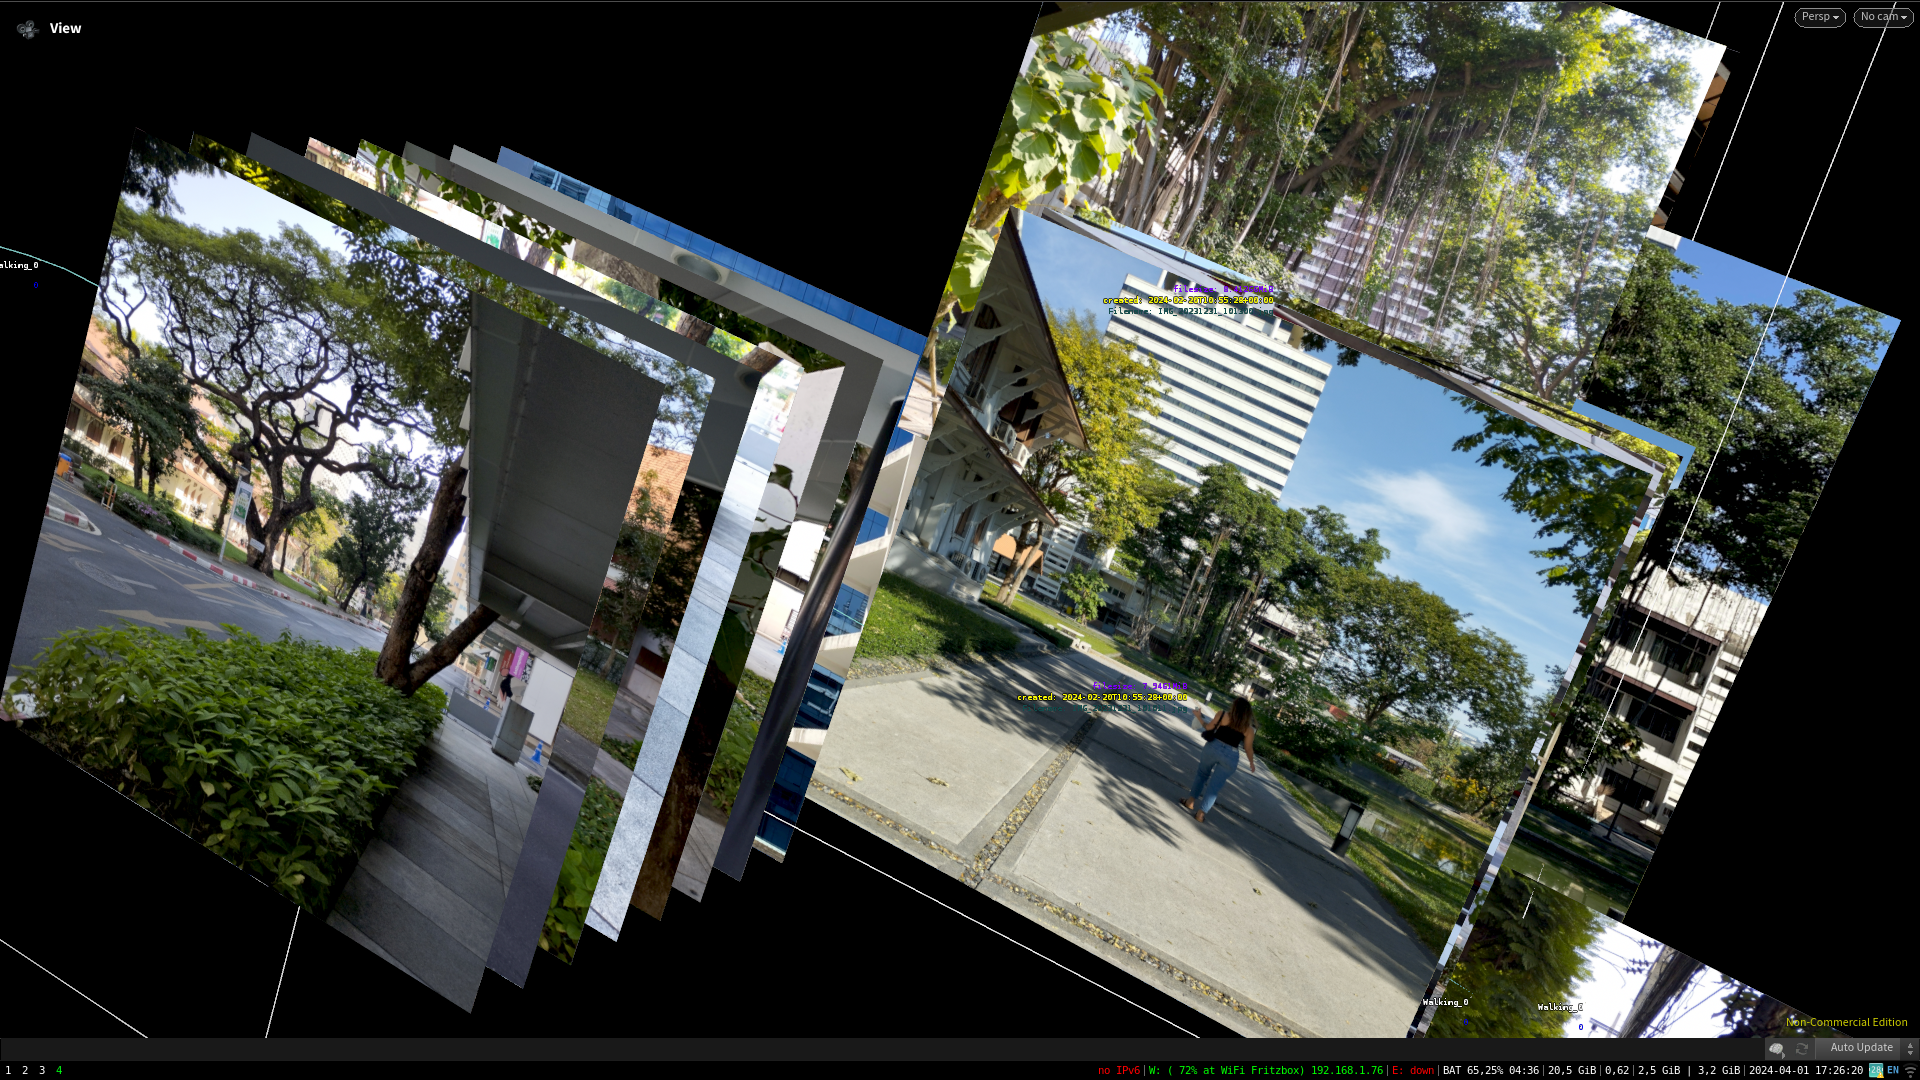
\includegraphics[width=\textwidth]{media/mapping_bkk2.png}
\end{figure}


\newpage
\section {video to 3D Model}

In this workshop, we covered how to generate a 3D model from a video of a
subject. In this case, this was the Sora AI video published from OpenAI. For
the assignment, the following is expected.

\begin{itemize}
	\item Generate one or more photogrammetry models from a
video/livestream/webscraped/Google Images/YouTube. Take footage related to your
projects.  
\item Reconstruct your camera path.
\item Find a way of adding information to the subject.
(Volume speculation, curvature, segmentation, etc.)
 \item Visualize your
model as a collection of images/renders.

	\item A short description of the procedure. 
\end{itemize}


\begin{figure}[h]
	  \centering
	  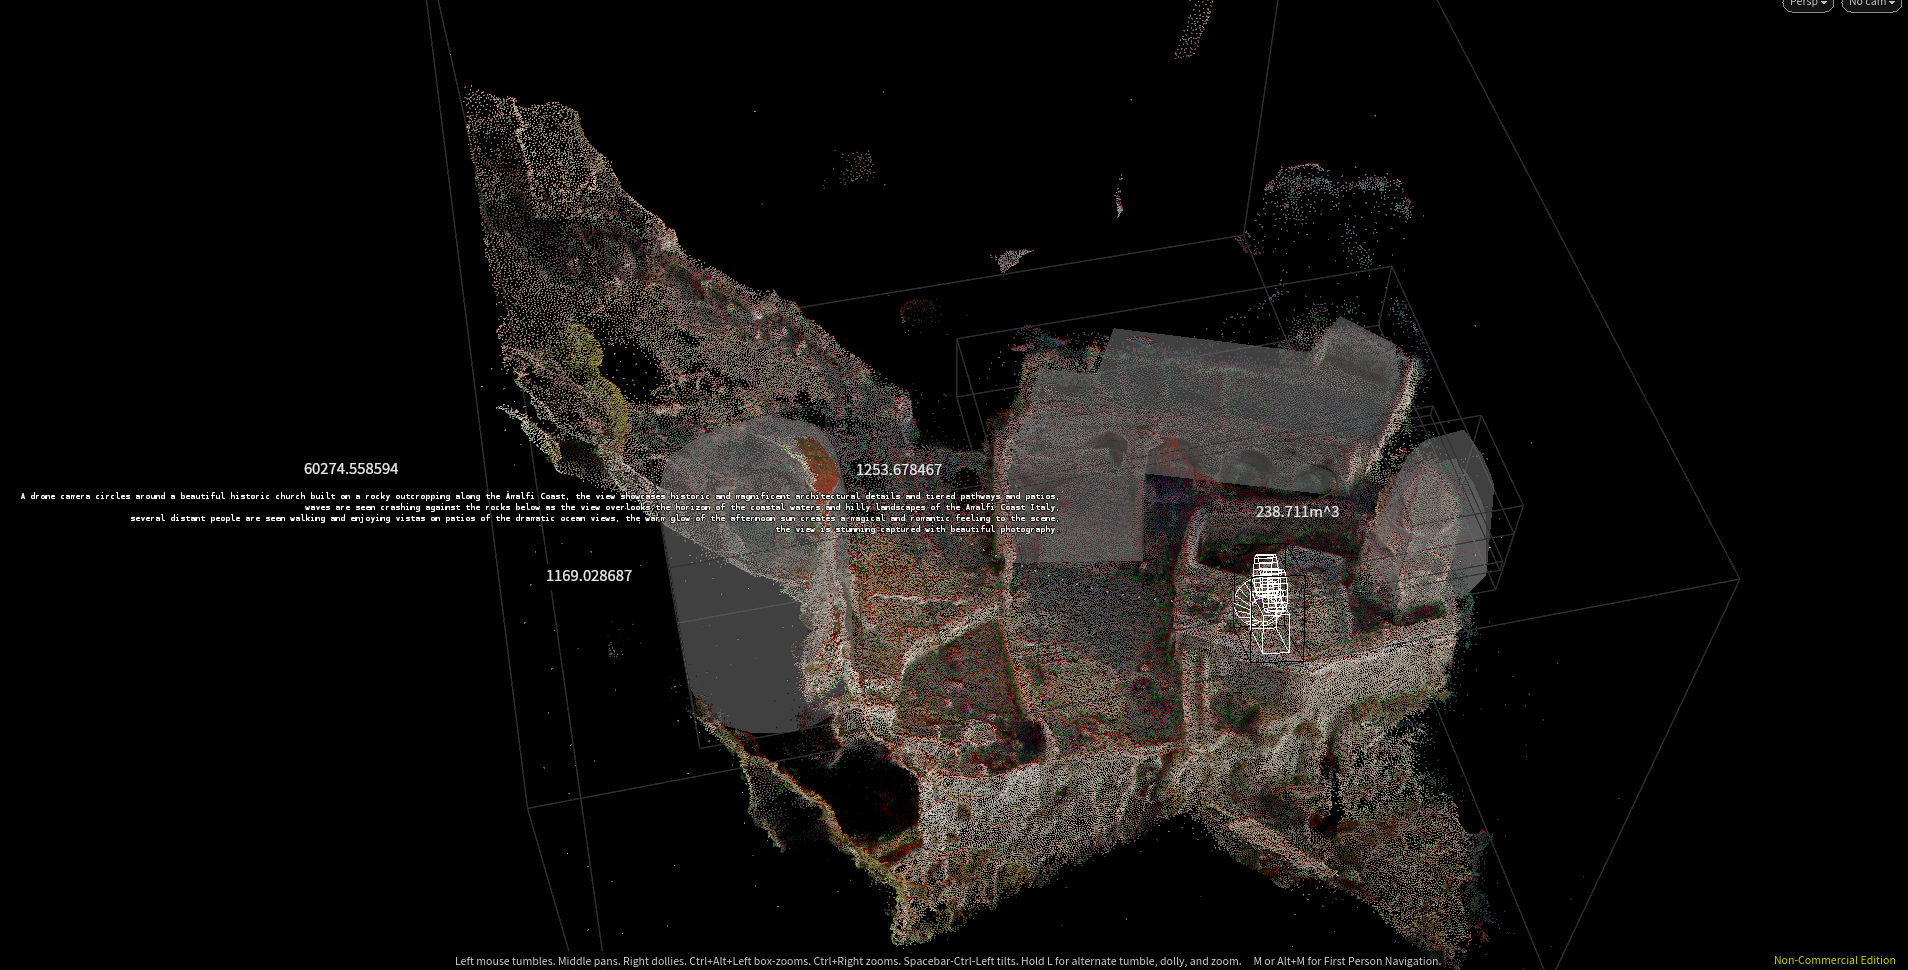
\includegraphics[width=\textwidth]{media/sora.png}
\end{figure}



\newpage
\section {Visualizing JSON in Houdini}

In this workshop, we covered how to generate a JSON file that can be read and
processed in Houdini. This is useful if you are constructing a .pickle or JSON
file and want to know how this can be visualized in Houdini. The following is
expected for the assignment.

\begin{itemize}
	\item
Based on your project and other workshops, visualize and produce a JSON file.
This can take many forms. It is up to you how to showcase this in the best way.
Please also include a snippet of your JSON file.  \end{itemize}

\begin{figure}[h]
	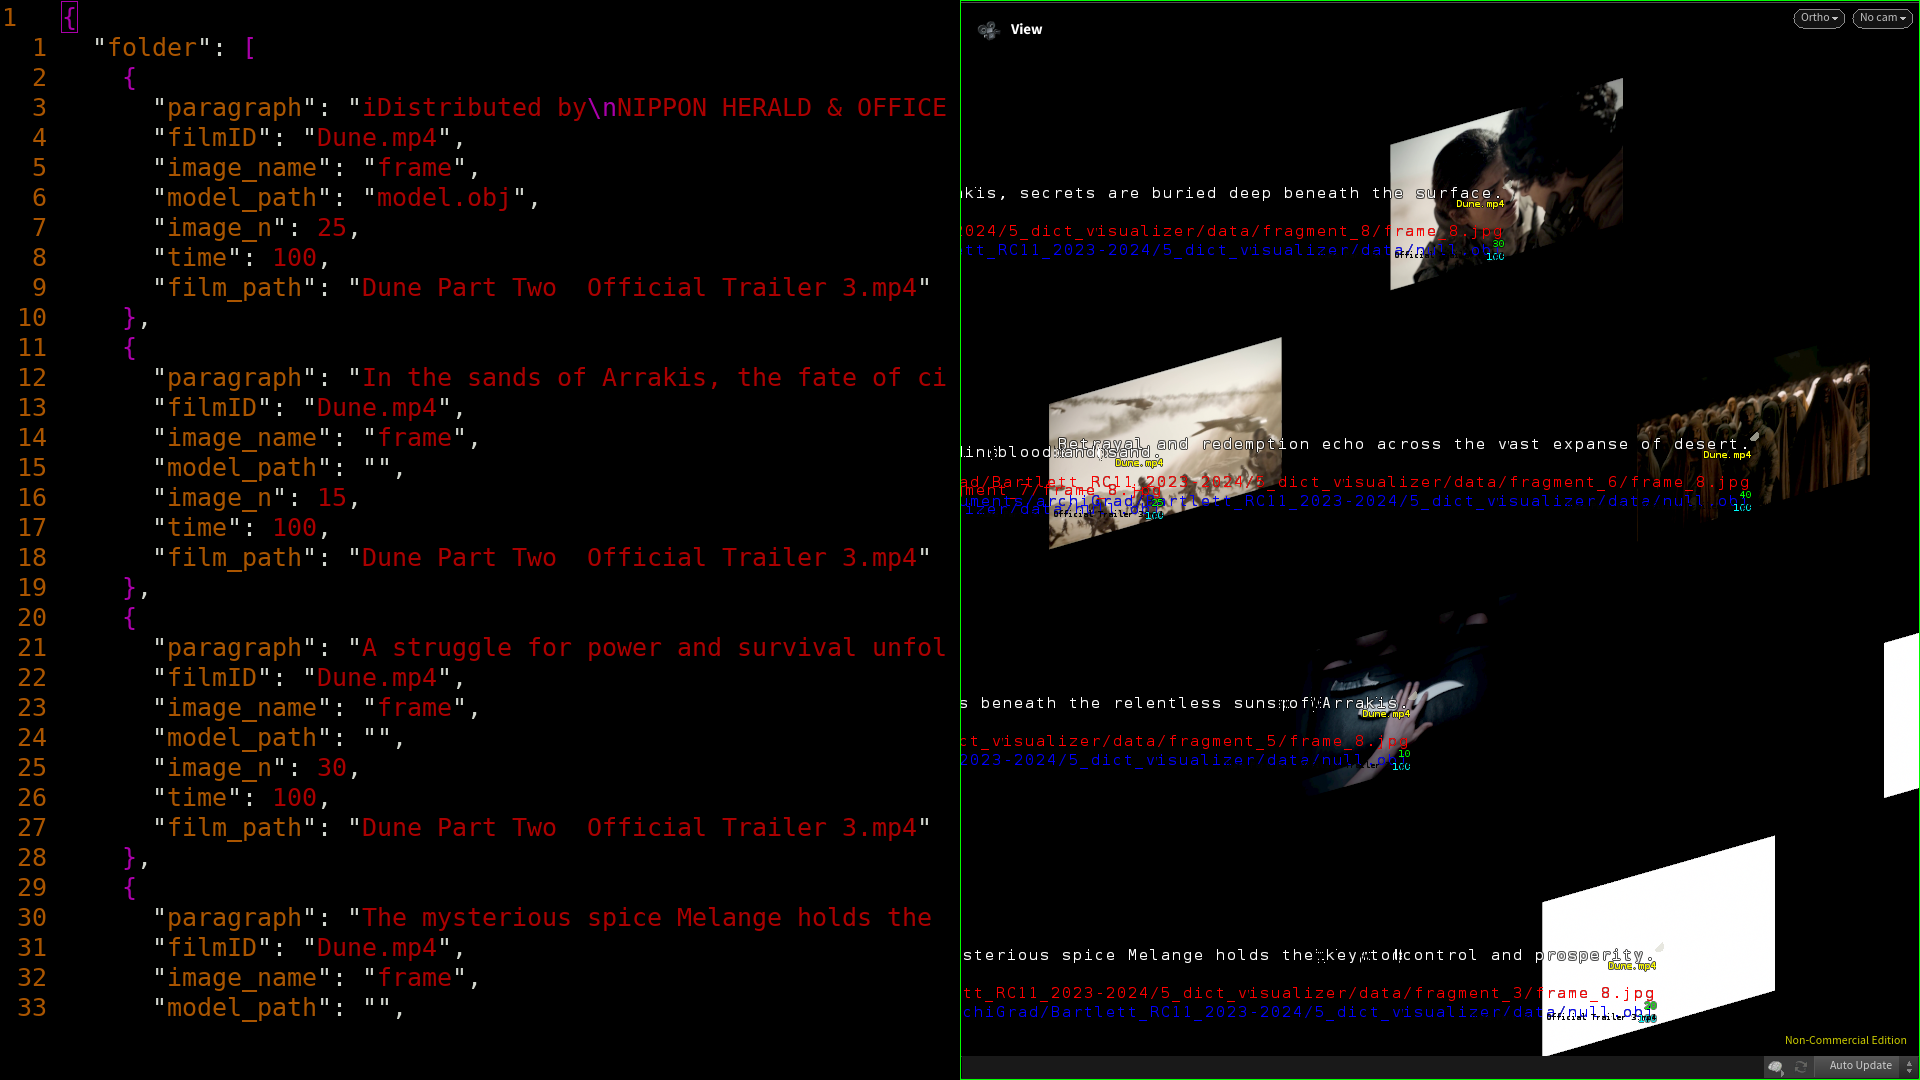
\includegraphics[width=\textwidth]{media/json_visualizer.png}
\end{figure}



\end{document}
